% ===== 原文 pp.77–79（PDF p.87–89） =====
% [原文 p.77]
\begin{figure}[htbp]
\centering
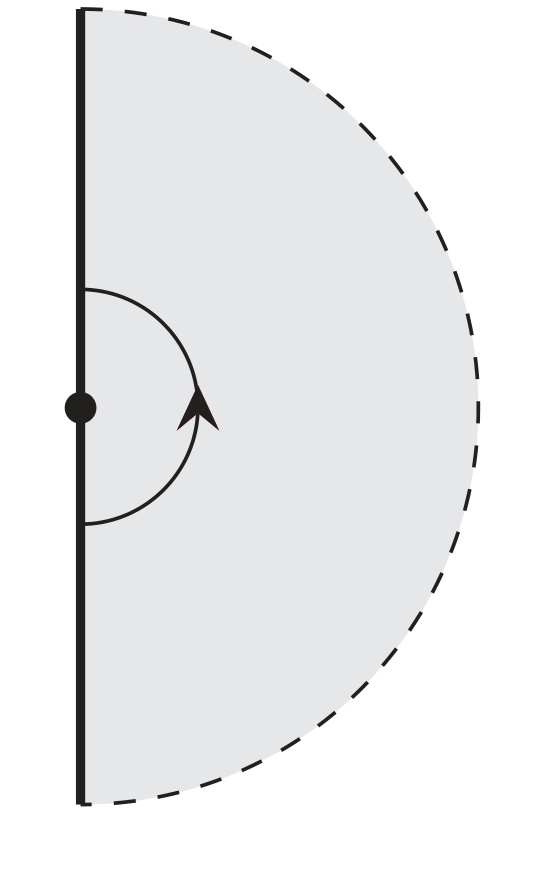
\includegraphics[width=0.4\textwidth]{fig61.png}
\figtitle{6.1}{摩天层对应于这样的边界线算子：沿其周围的一个小半圆，$A+\ii\phi$ 的和乐固定。圆点标出该边界线算子的位置，这里我们是在横截面上看它。}
\end{figure}

% [Tutor Note: 图 6.1 的读法：灰色圆盘是边界（3d 时空边界的横截面），黑点是坐在边界上的边界线算子，虚线半圆的两端落在边界上，弧线箭头表示沿该半圆取联络 $A+\ii\phi$ 的和乐。该和乐取值于 $\C^*$，正是 p.76 所说的 $\C^*$ 坐标；摩天层（固定和乐）因此对应边界线算子。]

镜像对称把 $\C^*$ 上的摩天层映到 $T^*S^1$ 的一个拉格朗日子流形，后者是 $S^1$ 上一个闭 1-形式 $\alpha$ 的图。从拓扑上看，这个子流形是一个圆，并带有一个平凡线丛配以平坦酉联络。这类对象的模空间是 $\C^*$：对 $\lambda\in\C^*$，$\lambda$ 的相位决定该酉联络的和乐，而 $\lambda$ 的绝对值决定 $\alpha$ 在 $S^1$ 上的积分。因此 B-侧的单位对象镜像于 $T^*S^1$ 的零截面配以平凡的平坦联络。为描述 A-侧的幺半结构，最好回顾 Nadler [42] 的一个定理：$T^*X$ 的（某个版本的）Fukaya-Floer 范畴等价于 $X$ 的可构造导出范畴。回忆一下：实流形 $X$ 上的可构造层是指在 $X$ 的某个 Whitney 分层的各层（strata）上局部常值的层；这样的层可以看作平坦联络的推广。可构造导出范畴的对象是上有界复形，其层上同调是可构造的。可构造导出范畴有一个由层复形的张量积给出的显然幺半结构。局部常值函数层是关于这个幺半结构的单位对象。根据 [43, 42]，这个对象对应于 $T^*S^1$ 的零截面配以平凡的平坦联络。这提示 A-侧的幺半结构由可构造导出范畴上的张量积给出。容易核对，这与镜像对称作用在 $\C^*$ 上摩天层的方式相容。

% [Tutor Note: p.77 “闭 1-形式的图是 Lagrangian 子流形”：若 $\alpha$ 是 $S^1$ 上的闭 1-形式，则其图 $\{(x,\alpha_x)\}\subset T^*S^1$ 上辛形式的拉回是 $\pi^*\dd\alpha=0$（$\dd\alpha=0$），故该图是 Lagrange 的；反之若 $\alpha$ 非闭，其图就不是 Lagrange 子流形。这解释了为什么摩天层的镜像是“闭” 1-形式的图，而不是任意 1-形式的图。]

% [Tutor Note: p.77 的 Nadler 定理（[42]）与 “$X$ 为单点” 的核对：当 $X$ 为单点时，可构造导出范畴退化为有限维向量空间复形的范畴，而 $T^*(\text{pt})$ 的 Fukaya-Floer 范畴相应退化；这与 §A.1 中 A-型 2d 规范理论在 $\C[2]$ 上的膜范畴为 $D^b(\mathrm{Coh}(\C[2]))$ 的说法一致。]

我们可以尝试把规范扇区与物质扇区合在一起。在 B-侧，我们有以 $\C^*\times\C[2]$ 为靶空间的 B-模型，其膜的范畴是 $D^b(\mathrm{Coh}(\C^*\times\C[2]))$。在 A-侧，我们有以 $T^*S^1$ 为靶空间的 A-模型与规范群为 $U(1)$ 的 A-型 2d 规范理论的张量积。人们可能猜测相应的膜范畴是 $T^*S^1$ 的 Fukaya-Floer 范畴的 $U(1)$-等变版本。更一般地，人们可能猜测：以 $T^*X$ 为靶空间的 A-模型与 A-型 2d $U(1)$ 规范理论作张量积后，其膜范畴是 $T^*X$ 的 Fukaya-Floer 范畴的 $U(1)$-等变版本。我们不清楚如何在数学上定义这样的等变 Fukaya-Floer 范畴。

% [原文 p.78]
根据 [43, 42] 的结果，一个自然的猜想是 $X$ 上层的等变可构造导出范畴。作为检验，注意当 $X$ 为单点时，$U(1)$-等变可构造导出范畴等价于 $D^b(\mathrm{Coh}(\C[2]))$ [28]。而如前所述并在附录 A 中解释的，这确实就是 A-型 2d 规范理论的膜范畴。其幺半结构似乎是标准的那一个（导出张量积）。另一方面，在 B-侧，幺半结构则是 $\C[2]$ 上凝聚层的张量积与 $\C^*$ 上卷积乘积的组合。

\subsubsection{DN 条件}

接着考虑 A-侧这样的边界条件：规范扇区取 Dirichlet 条件，而物质扇区中 $A_4$ 取 Neumann 条件。它对偶于 B-型规范扇区的 Dirichlet 条件，以及以 $T^*[2]\C^*$ 为靶空间的 RW 模型中令 $\sigma=0$、而让复标量 $\tau=A_4+\ii\phi_4$ 自由涨落的边界条件。

在 B-侧，区间上的约化给出以 $\C^*\times\C^*$ 为靶空间的 B-模型，因此边界线算子的范畴是 $D^b(\mathrm{Coh}(\C^*\times\C^*))$。在 A-侧，约化给出以 $T^*U(1)\times T^*U(1)$ 为靶空间的 A-模型，因此边界线算子的范畴是 Fukaya-Floer 范畴。这两个范畴由通常的 2d 镜像对称而等价。幺半结构在 B-侧最容易确定。它既不是导出张量积，也不是卷积，而是二者的组合。出现这种情况是因为两个 $\C^*$ 的来源非常不同：其中一个来自 3d B-型规范理论，另一个来自以 $T^*[2]\C^*$ 为靶空间的 Rozansky-Witten 模型。

\subsubsection{ND 条件}

最后我们考虑 A-侧这样的边界条件：规范扇区取 Neumann 条件，而 $A_4$ 取 Dirichlet 条件。这正是对应于 $t=1$ 时 Gukov-Witten 面算子的情形。事实上，$A_4$、$\phi_4$ 与 $\phi_3$ 的 Dirichlet 条件意味着 $A$ 的和乐固定，而 1-形式 $\phi$ 具有如下形式的奇异性
\[
  \beta\frac{\dd r}{r}-\gamma\,\dd\theta,
\]
其中 $-\gamma$ 是 $\phi_4$ 的边界值，$\beta$ 是 $\phi_3$ 的边界值。$A_4$ 的边界值是 Gukov-Witten 参数 $\alpha$。规范扇区的 Neumann 条件还依赖于边界 theta 角，它对应于 Gukov-Witten 参数 $\eta$。如上所述，$A_4$ 与 $\phi_3$ 的边界值其实是不相关的。这与 [2] 的结果一致：那里证明了在 $t=1$ 时参数 $\alpha$ 与 $\beta$ 是不相关的。因此 A-侧该面算子真正的参数空间是 $\C^*$。

% [Tutor Note: p.78 的 Gukov-Witten 参数对应关系容易记错：此处 $-\gamma$（带负号）是 $\phi_4$ 的边界值，$\beta$ 是 $\phi_3$ 的边界值，$\alpha$ 是 $A_4$ 的边界值，$\eta$ 是边界 theta 角。核对方法：按 §6.1，对阿贝尔群有 $\alpha\in U(1)$、$\beta,\gamma\in\R$、$\eta\in U(1)$；$t=1$ 时 $\alpha,\beta$ 不相关（[2]），故面算子的参数空间是 $(\gamma,\eta)\in\R\times S^1\simeq\C^*$，而 $t=\ii$ 时（p.79）相关参数是 $(\alpha,\gamma)\in S^1\times\R\simeq\C^*$、不相关的是 $\beta,\eta$。两组“相关参数”的差别正是检验这里对应关系是否写反的锚点。]

% [原文 p.79]
电磁对偶把 DD 条件映为 B-型规范理论的 Neumann 条件，以及 RW 模型中固定 $\tau$、让 $\sigma$ 自由涨落的边界条件。后一边界条件依赖于场 $\tau=A_4+\ii\phi_4$ 的边界值。从 4d 的观点看，这个边界值编码了 Gukov-Witten 参数 $\alpha$ 与 $\gamma$。如 [2] 所解释的，它们是在 $t=\ii$ 时的相关参数。B-型规范理论中的 Neumann 边界条件也有两个参数（$\phi_3$ 的边界值与边界 theta 角），它们对应于 Gukov-Witten 参数 $\beta$ 与 $\eta$。但如上所述、并在 [2] 中从另一观点说明的，这些参数在 $t=\ii$ 时是不相关的。

让我们比较 3d 边界线算子的范畴，从 4d 的观点看它们被解释为坐在 Gukov-Witten 面算子上的线算子的范畴。在 B-侧，区间上的约化给出以 $\C[2]$ 为靶空间的 B-模型与一个 B-型 2d 规范理论的张量积，因此边界线算子的范畴是 $D^b_{\C^*}(\mathrm{Coh}(\C[2]))$。在 A-侧，区间上的约化给出 A-型 2d 规范理论与以 $T^*\R$ 为靶空间的修正 A-模型的张量积。其膜范畴是 A-型 2d 规范理论边界条件范畴的一个修正版本：其中边界自由度的空间带有来自周期标量 $A_4$ 缠绕的额外整数分次，且态射要求关于该分次为次数零。由于 A-型 2d 规范理论中的膜可以等同于 $D^b(\mathrm{Coh}(\C[2]))$ 的对象，组合系统的边界条件范畴等价于 $D^b_{\C^*}(\mathrm{Coh}(\C[2]))$，与我们在 B-侧得到的结果一致。

\subsection{\texorpdfstring{$t=1$}{t=1} 时面算子 2-范畴的一个猜想}

仿照 Rozansky-Witten 模型的情形，人们可以猜测：$t=1$ 时面算子的 2-范畴可以用特定边界条件（NN 条件）下边界线算子的幺半范畴上的模范畴来描述。我们在上面论证过，这个幺半范畴是 $S^1$ 的 $U(1)$-等变可构造导出范畴，其中 $U(1)$ 在 $S^1$ 上的作用平凡。或许更好的做法是把它看成 $S^1$ 上的一个 $U(1)$-等变幺半 DG-范畴层。我们可以给每个面算子关联一个层，它是该 $U(1)$-等变幺半范畴层上的 $U(1)$-等变模范畴层；我们猜测这个对应是 2-范畴的等价。Gukov-Witten 型算子对应于 $S^1$ 上的摩天层。

于是电磁对偶蕴含：这个 2-范畴与 $\C^*$ 上相干的 $\C^*$-等变导出范畴层所成的 2-范畴等价。

% [Tutor Note: p.79 用“模范畴”而非“范畴”来描述 2-范畴的理由：给定边界条件 $X_0$（此处为 NN 条件）后，任意面算子 $X$ 上的线算子范畴 $\cV_{XX_0}$ 是幺半范畴 $\cV_{X_0X_0}$ 上的模范畴，且 [36] 提议该模范畴完全刻画面算子。RW 模型的先例是：以 $T^*[2]\C^*$ 为靶空间的 RW 模型的边界条件 2-范畴等价于 $D^b(\mathrm{Coh}(\C^*))$ 上模范畴的导出 2-范畴，即 Toën-Vezzosi 意义下 $\C^*$ 上的导出范畴层 [44]。本节只是把 $D^b(\mathrm{Coh}(\C^*))$ 换成 NN 条件下的幺半范畴。]

% [Tutor Note: p.79 Gukov-Witten 型算子对应 $S^1$ 上的摩天层，可与 p.76–77 的结论交叉核对：Gukov-Witten 面算子在 $t=1$ 时的参数空间是 $\C^*$（p.78），而 $S^1$ 上摩天层的模空间也是 $\C^*$（p.77：相位给和乐、模长给 $\alpha$ 的积分）；两侧参数个数与结构一致，可作为该猜想的自洽性检验。]
